%% 
%% Copyright 2007, 2008, 2009 Elsevier Ltd
%% 
%% This file is part of the 'Elsarticle Bundle'.
%% ---------------------------------------------
%% 
%% It may be distributed under the conditions of the LaTeX Project Public
%% License, either version 1.2 of this license or (at your option) any
%% later version.  The latest version of this license is in
%%    http://www.latex-project.org/lppl.txt
%% and version 1.2 or later is part of all distributions of LaTeX
%% version 1999/12/01 or later.
%% 
%% The list of all files belonging to the 'Elsarticle Bundle' is
%% given in the file `manifest.txt'.
%% 
%% Template article for Elsevier's document class `elsarticle'
%% with harvard style bibliographic references
%% SP 2008/03/01

%\documentclass[preprint,12pt,authoryear]{elsarticle}  %default in the template
%\documentclass[preprint,10pt,authoryear]{elsarticle}

%% Use the option review to obtain double line spacing
%% \documentclass[authoryear,preprint,review,12pt]{elsarticle}

%% Use the options 1p,twocolumn; 3p; 3p,twocolumn; 5p; or 5p,twocolumn
%% for a journal layout:
%% \documentclass[final,1p,times,authoryear]{elsarticle}
%% \documentclass[final,1p,times,twocolumn,authoryear]{elsarticle}
 \documentclass[final,3p,times,authoryear]{elsarticle}
%% \documentclass[final,3p,times,twocolumn,authoryear]{elsarticle}
%% \documentclass[final,5p,times,authoryear]{elsarticle}
%% \documentclass[final,5p,times,twocolumn,authoryear]{elsarticle}

%% For including figures, graphicx.sty has been loaded in
%% elsarticle.cls. If you prefer to use the old commands
%% please give \usepackage{epsfig}

%% The amssymb package provides various useful mathematical symbols
\usepackage{amssymb}
%% The amsthm package provides extended theorem environments
 \usepackage{amsthm}
 \usepackage{amsmath}
 \usepackage{color}
 \usepackage{amsmath}
\usepackage{siunitx}
\usepackage[]{algorithm2e}


\usepackage{framed} % Framing content
\usepackage{multicol} % Multiple columns environment
\usepackage{nomencl} % Nomenclature package
\makenomenclature
%\setlength{\nomitemsep}{-\parskip} % Baseline skip between items
\setlength{\nomitemsep}{0.01cm}
\renewcommand*\nompreamble{\begin{multicols}{2}}
\renewcommand*\nompostamble{\end{multicols}}
\newcommand{\degreeC}{\ensuremath{^\circ}C }

\usepackage[nonumberlist]{glossaries}
\makeglossaries 


%% The lineno packages adds line numbers. Start line numbering with
%% \begin{linenumbers}, end it with \end{linenumbers}. Or switch it on
%% for the whole article with \linenumbers.
%% \usepackage{lineno}

\journal{Urban Climate}


\begin{document}


%\include{TargetHtc_glossary} 


\begin{frontmatter}

%% Title, authors and addresses

%% use the tnoteref command within \title for footnotes;
%% use the tnotetext command for theassociated footnote;
%% use the fnref command within \author or \address for footnotes;
%% use the fntext command for theassociated footnote;
%% use the corref command within \author for corresponding author footnotes;
%% use the cortext command for theassociated footnote;
%% use the ead command for the email address,
%% and the form \ead[url] for the home page:
%% \title{Title\tnoteref{label1}}
%% \tnotetext[label1]{}
%% \author{Name\corref{cor1}\fnref{label2}}
%% \ead{email address}
%% \ead[url]{home page}
%% \fntext[label2]{}
%% \cortext[cor1]{}
%% \address{Address\fnref{label3}}
%% \fntext[label3]{}

\title{Urban typologies through city block size and regularity}


%% use optional labels to link authors explicitly to addresses:


\author[melb]{Kerry~A.~Nice\corref{cor1}}
\ead{kerry.nice@unimelb.edu.au}
\author[melb]{Gideon D.P.A. Aschwanden\corref{cor1}}
\ead{gideon.aschwanden@unimelb.edu.au}
\author[melb,sun]{Jason Thompson}
\author[melb]{Jasper S. Wijnands}
\author[melb]{Michele Acuto}
\author[melb]{Haifeng Zhao}
\author[melb,pop]{Mark Stevenson}
\author[melb]{Jingcheng Wang}

\cortext[cor1]{Principal corresponding author}
\address[melb]{Transport, Health, and Urban Design Hub, Faculty of Architecture, Building, and Planning, University of Melbourne, Victoria, Australia}
\address[sun]{Centre for Human Factors and Sociotechnical Systems, University of the Sunshine Coast, Australia}
\address[pop]{Melbourne School of Engineering; and Melbourne School of Population and Global Health, University of Melbourne, Victoria, Australia}

The method is robust in detecting similarities between cities but between neighbourhoods of different cities. This opens the opportunity to investigate the mechanics and implications of cities structures on a unprecedented level of disaggregation where the energy, emission, health and economic implications of city design are evaluated on a 800x800m grid, your neighbourhood.


\begin{abstract}

As cities grow and evolve, the road networks and urban block structure provides clues as to the process and governance under which this growth occurred. We propose a novel quantitative and objective method to discover city typologies on the neighborhood scale of street patterns, city block size and regularity. This follows \cite{Louf2014a}'s finding that a systematic quantitative method to identify different neighborhoods is currently lacking. 

Our method 800m x 800m samples of custom abstract / stylized maps from Google Maps of the world's largest 1692 cities. Using a floodfill, the size and regularity of each city blocks in a samples is calculated and histograms constructed for each map sample. A self organising map (SOM), that deploys an unsupervised learning algorithm is used, for feature detection and to cluster (arrange) these images into city block typologies. 


\end{abstract}

\begin{keyword}
urban typologies, self organizing map, unsupervised learning algorithm, urban design, urban planning, city clustering
%% keywords here, in the form: keyword \sep keyword

%% PACS codes here, in the form: \PACS code \sep code

%% MSC codes here, in the form: \MSC code \sep code
%% or \MSC[2008] code \sep code (2000 is the default)

\end{keyword}

\end{frontmatter}







\section{Introduction}\label{sec:introduction}

%% Why is understanding the city so important
%% - Health (Lancet)
%% - Transport (Space Syntax)
%% - Economics (Urban Economics)

\subsection{City Typologies}\label{sec:introduction2}
Cities are the most complex entities humans have ever created, but they are examples of 'organised complexity' that allow us to discerne some kind of order within the diversity and complexity cities present \citep{Kropf2014}. Approaches that aim to classify the built form are using a hirarchitcal dichotomy based on the scale of urban element. Different scales of dichotomies exist from 3 to 6 steps and range in scale from the building material to the territorial organisation of cities  \citep{Lynch1981} \citep{Conzen1960} \citep{Caniggi1979} \citep{Castex1980} \citep{Mouden1988} \citep{Allain2004}.

(insert figure with different scales todo GA xxx)

The used elements by the existing approaches are not coherant, some are using going to the level of rooms, others are expanding on the larger scale. One of the few consistant elements used by all existing approaches is the "Street Block", "Block", "Urban Tissue" or "insula", the area that is confined by the surrounding streets may it be build up, open space or a combination of both.
The evaluation and classification based on the individual dichotomy is 



\section{Methods}\label{sec:Methods}

\subsection{Imagery sampling}\label{sec:methods2}
The concept employed in this study was to sample maps of individual cities, calculate block size and regularity, and then use a self organizing map (SOM) to cluster different urban types.

1692 cities with populations $>$ 300,000 people were initially selected for analysis \citep{UN2014}. Data from Google Maps was used to identify urban form for each city in a globally consistent framework. The sampling area for each city was chosen as a circular area aligned to the city's centre, where the radius $r$ (km) of the sampling area was determined based on the population size $p$ according to \citet{Barthelemy2016}: 

\begin{equation}
r = \sqrt{ \frac{28.27}{\pi} \bigg( \frac{p}{300,000}  \bigg)^{0.85} }
\end{equation}


Having identified individual cities, a two-stage sampling approach was applied. As no standardised urban boundaries are available for all the cities evaluated in this study, a methodology had to be developed to define these. Firstly, a sampling area extending 1.5 km from the identified city centroid \citep{UN2014} was set as a baseline. As sample cities' populations increased in size, the sampling area increased by a power of 0.85 to the proportional increase in population size \citep{Barthelemy2016}. Standardising the sampling area in this manner avoided socio-political discrepancies relating to a city's `true' boundary and captured differences in population density and shape between small (e.g., Wellington, New Zealand; Izmit, Turkey) and global mega-cities (e.g., Tokyo, Japan;  Delhi, India). Location sampling areas were adjusted for the earth's curvature \citep{Sinnott1984}. Large water-bodies (e.g., oceans but not coastlines) were removed from the sampling area, as they were not indicative of urban form . 

These procedures result in a population and water body-adjusted circular area centred on the city's central coordinates, capturing the widest extent of each city while minimising the amount of non-urban locations. For example, Figure \ref{fig:parissample} shows the resulting sampling locations used in collecting imagery for Paris. 

\begin{figure}[!htbp]
    \centering    
\includegraphics[scale=0.5]{Images/Paris-StreetView-SampleLocations_crop.png}  
\caption{\bf Sampling locations for map imagery (from Paris, France) \citep{GoogleStatic2017}.}    
 \label{fig:parissample}  
\end{figure} 



\subsection{Imagery sources}\label{methodsimagery}
Imagery used was Google Maps images. Images were sized 320 by 320 pixels using a zoom level of 16 (approximately 800x800m at the equator to 450x450m at higher latitudes). These were obtained from the selected locations using a custom style defined with the Google Static Maps API \citep{GoogleStatic2017} (see Figure~\ref{fig:maps} for examples of Paris, France). The images provide a high-level abstraction of road (black) and public transport (orange) networks, green space (green), and water bodies (blue). Any remaining space is coded white. Due to mapping inconsistencies in South Korea, all 25 South Korean cities were removed from the dataset, reducing the number of cities to 1665. 1000 training images were used per city. In addition, to enable in depth case studies, maps were sampled for Melbourne and Sydney, Australia at a 400m grid resolution across the greater metropolitan areas. This results in an additional 23,027 locations for Melbourne and 24,596 for Sydney. As a result, the total dataset consists of 1,714,591 images.



\begin{figure}[!htbp]
    \centering    
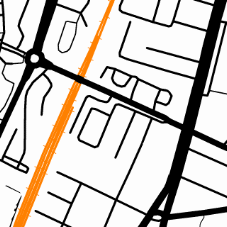
\includegraphics[scale=0.7]{Images/Map1.png}  
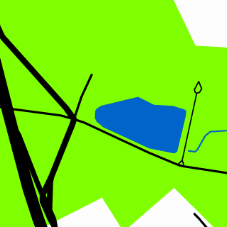
\includegraphics[scale=0.7]{Images/Map2.png}
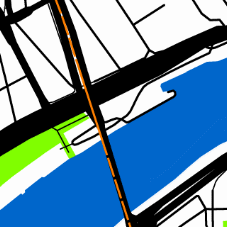
\includegraphics[scale=0.7]{Images/Map3.png}
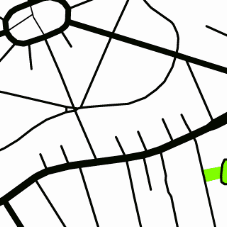
\includegraphics[scale=0.7]{Images/Map4.png}
\caption{\bf Four sample Google Maps training data images (from Paris, France) \citep{GoogleStatic2017}.}    
 \label{fig:maps}  
\end{figure} 


\subsection{Calculating block size and regularity}\label{methodscalc}

Block size and regularity were calculated for each sampled image with the following algorithm, using Java 8 \citep{Oracle2018}:

\begin{algorithm}[H]
\SetAlgoLined
\KwResult{List of region sizes and region regularity for an image stored in Sqlite3 database }
 Start at top left point of image\;
 \While{Locate next white pixel by iterating across rows and columns}{
  Floodfill area using boundaries of all non-white colors (i.e. black roads, green space, blue water)\;
  Count pixel size of region\;  
  Find x1 with the lowest x value\; 
  Find y1 with the lowest y value\;
  Find x2 with the highest x value\; 
  Find y2 with the highest y value\;
  Construct rectangle using the four vertices (x1,y1), (x1, y2), (x2,y1), (x2,y2)\;
  Floodfill the region outside the rectangle\;
  Count the number of pixels outside of the rectangle as measure of irregularity\;
  Add size and regularity counts to list for the image\;
 }
 Store list in database\;
 \caption{Calculation of block sizes and regularity}
\end{algorithm}


Sample results are shown in Figure \ref{fig:floodfilled}.

\begin{figure}[!htbp]
    \centering    
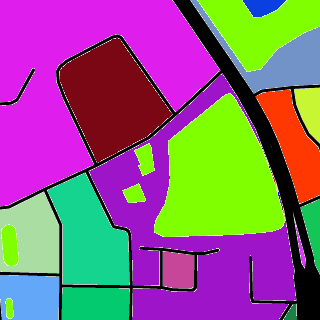
\includegraphics[scale=0.3]{Images/city82-745994-result.png}  
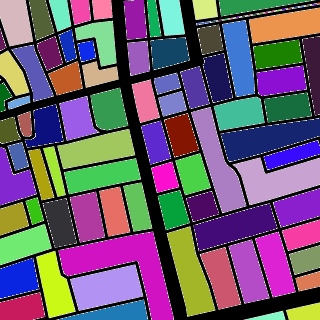
\includegraphics[scale=0.3]{Images/city1667-82612-result.png}
\caption{\bf Results of flood filled city blocks.}    
 \label{fig:floodfilled}  
\end{figure} 

\subsection{City regions histograms}\label{methodshist}

Using the region counts, histograms were constructed for each image. Two histograms were constructed for each image, one each for region sizes and region regularity. The histograms were sorted into 15 bins, the number of bins calculated by Sturges' formula \citep{Sturges1926}. In addition, to reduce the skewing of data towards the first bin, variable bins were used to spread this data across the remaining bins. The first bin starts with a size boundary of 1 and each following bin has a boundary of the current bin boundary times a multiplier. A multiplier of 2.3 was used to fit the maximum count size (320x320 pixels = 102400) into 15 bins.

Resulting histograms for sample map regions are shown in Figure \ref{fig:mapsandHist}. The histograms used in clustering the map regions are constructed by combining the 15 bins of region size frequencies (on the left side) with the 15 bins of region regularity (on the right) into a single histogram. 


\begin{figure}[!htbp]
    \centering    
\includegraphics[scale=0.34]{Images/{city169_5798_39.739486,-105.019810}.png}  
\includegraphics[scale=0.34]{Images/{city169_455115_39.737462,-105.021318}.png} 
\includegraphics[scale=0.34]{Images/{city169_59949_39.732605,-105.016022}.png} 
\includegraphics[scale=0.34]{Images/{city1521_754459_36.078403,-79.813528}.png} 
%\includegraphics[scale=0.25]{Images/{XX}.png} 
\\
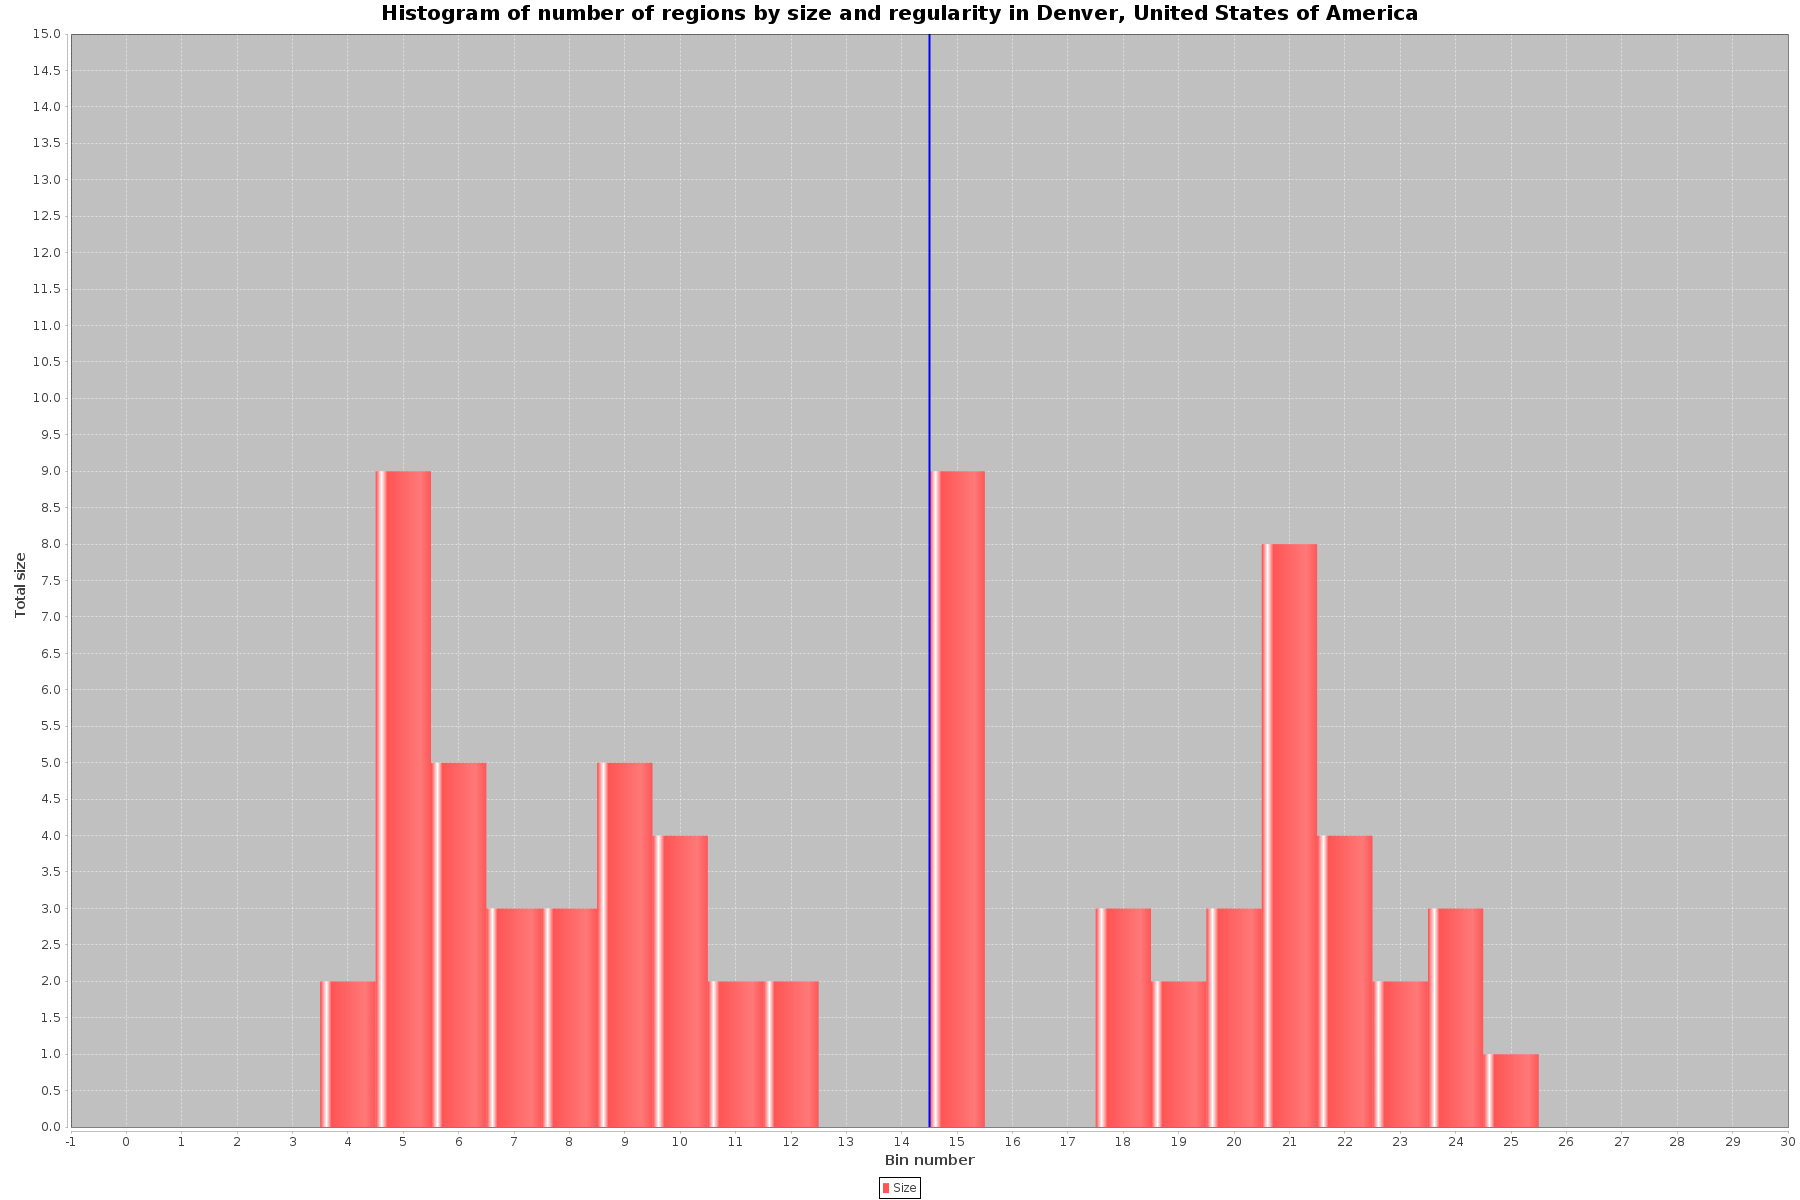
\includegraphics[scale=0.06]{Images/Combinedcity169-5798.png}
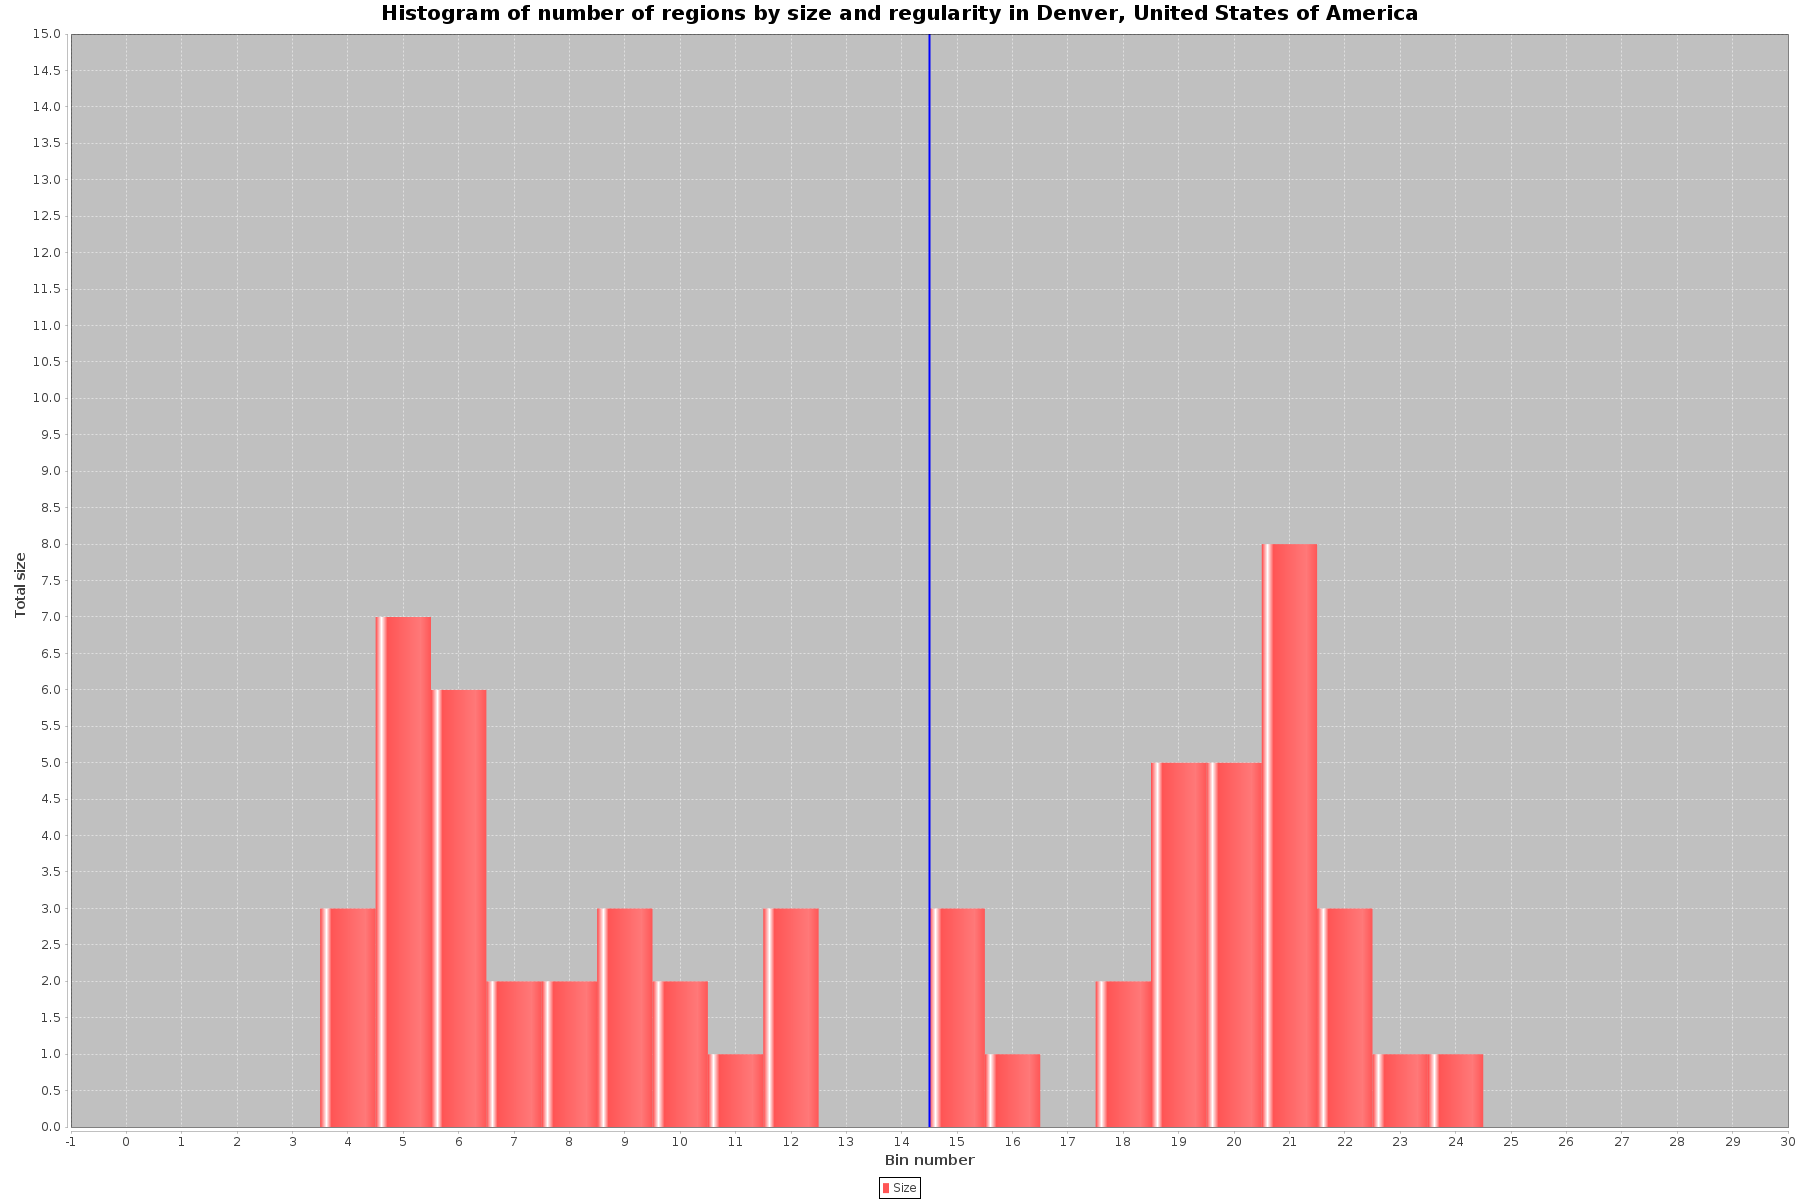
\includegraphics[scale=0.06]{Images/Combinedcity169-455115.png}
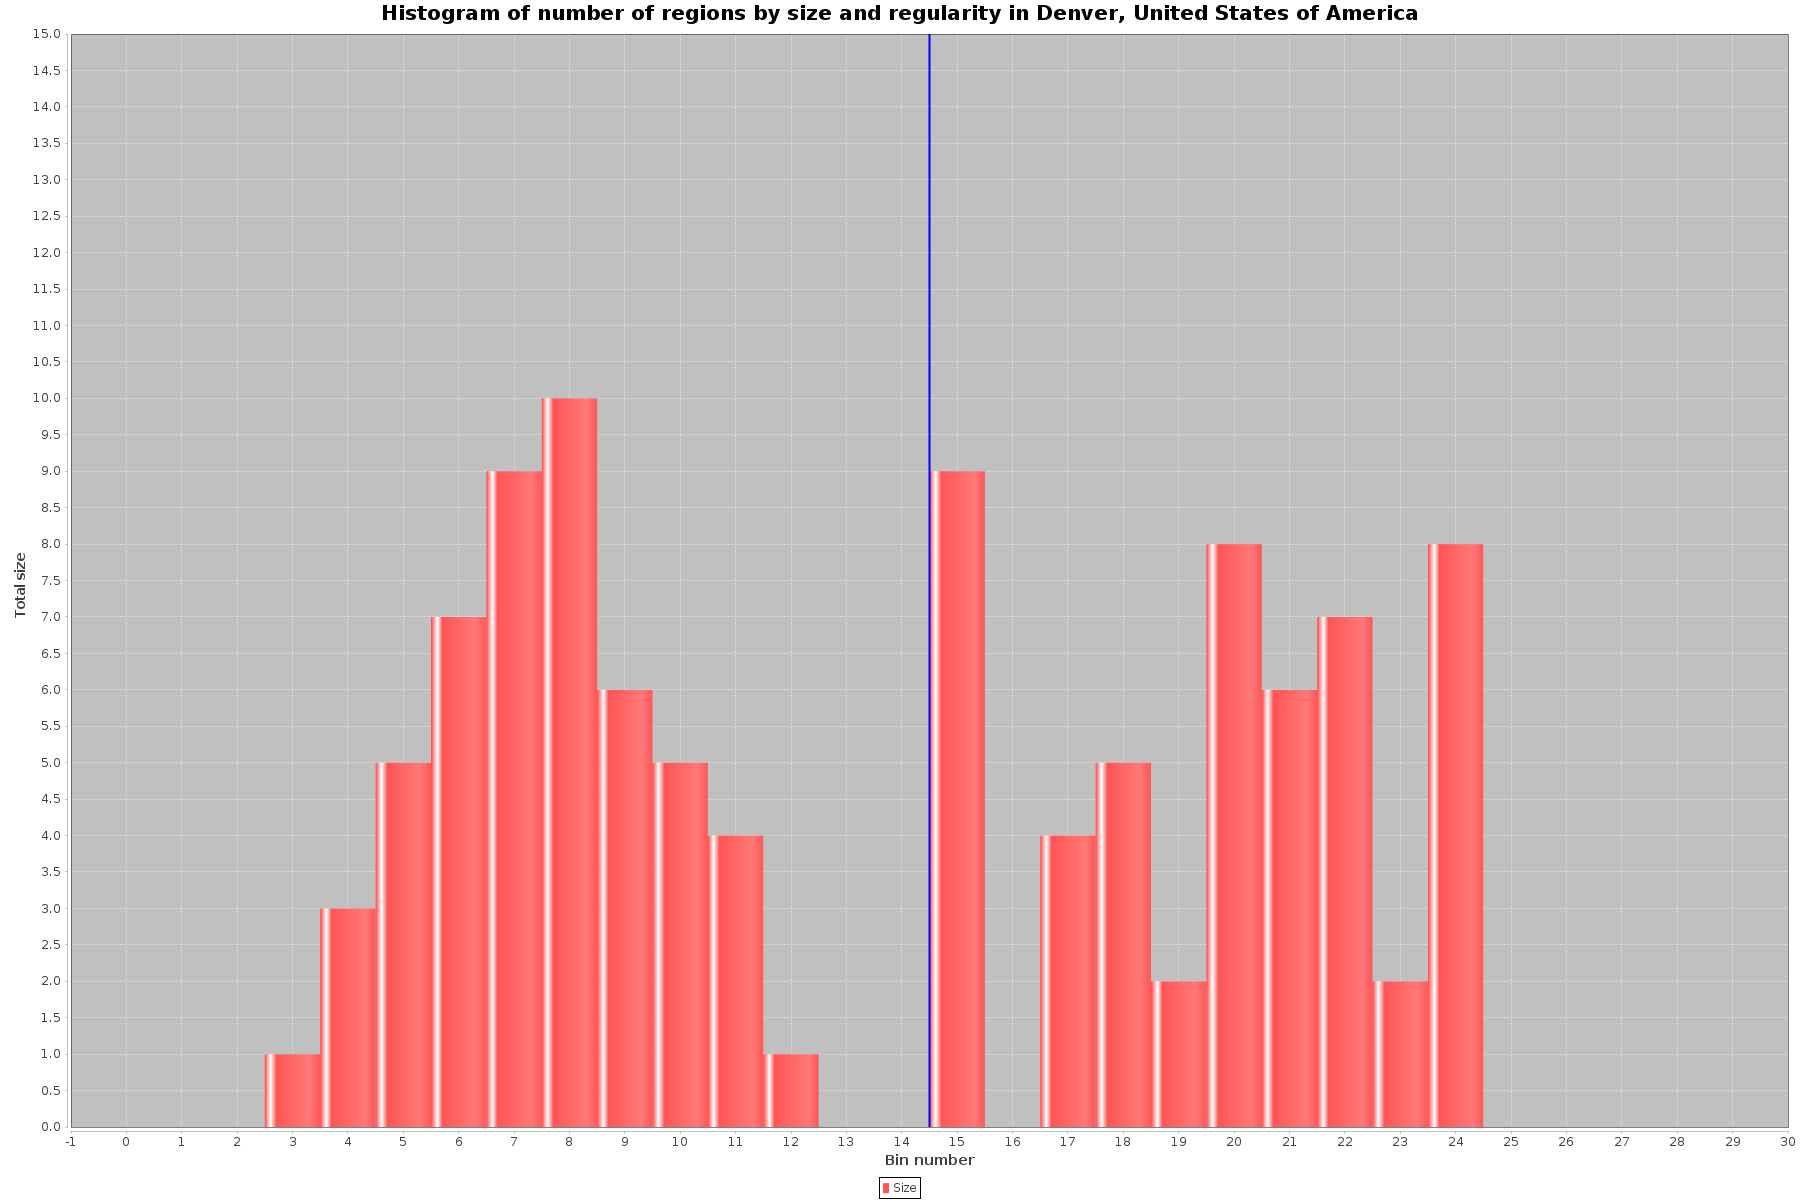
\includegraphics[scale=0.06]{Images/Combinedcity169-59949.png}
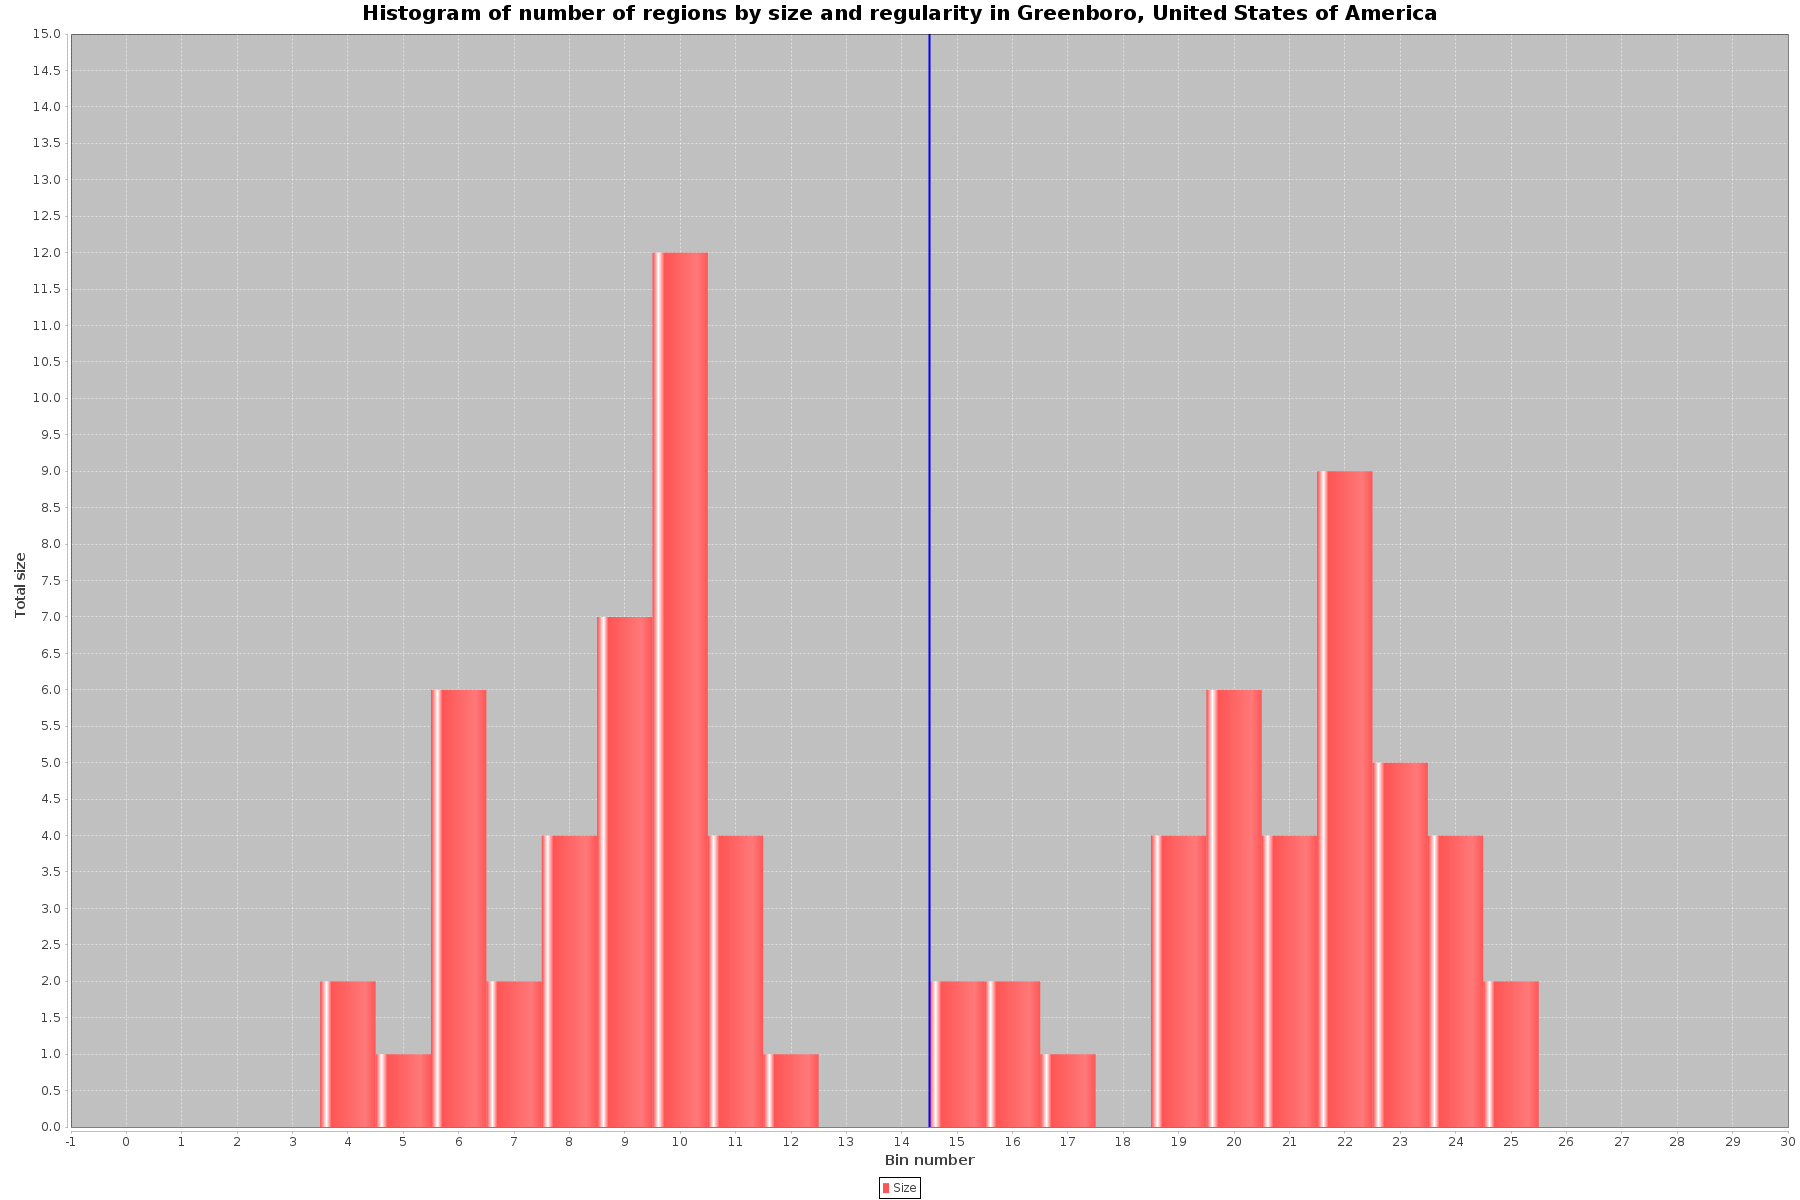
\includegraphics[scale=0.06]{Images/Combinedcity1521-754459.png}
%\includegraphics[scale=0.05]{Images/XX}
\caption{\bf Four samples of map regions (top) and resulting histograms (bottom). Region size and regularity are joined into a combined histogram, with size frequencies on the left side of the graph and regularity on the right.}    
 \label{fig:mapsandHist}  
\end{figure} 

\subsection{Similar city regions}\label{methodssimilarity}

\begin{figure}[!htbp]
\centering  
\caption{\bf Map of Melbourne overlayed with a grid of 23000 satelite images colourised according based on their location with in the SOM and {insert what colour schema is used}    
 \label{fig:clustermapsimages}  
\end{figure} 

\subsection{Clustering city regions}\label{methodscluster}
~1.7 million images histograms (1000 images each from 1665 cities) are clustered using a self organizing map (SOM), using Java 8 \citep{Oracle2018}.  
The SOM methodology \citep{Kohonen1982} is a data driven methodology that transforms a n dimensional data source into a lower dimensional space, mostly 2 dimensions why it is called a map, while keeping the typology of the high dimensional space intact. This transformation keeps the relative n-dimensional proximity of two datapoints intact when projecting them in the lower space. The distance in the lower dimensional representation is therefore a similarity index of the higher dimensional space. Each point in the 2 dimensional map has location (x,y) and is associated with a vector of values from the n-dimensional space (Vx,y = [v1,v2...n]).
The argument for the choice of this methodology lies in its ability to create two dimensional maps of smoothly changing patterns from the original high dimensional space. Additionally the SOM map spans the extremes observed in the original data and allows for investigation on how the data is distributed, potential paths between two observations or function approximation with non-linear relations \citep{Barreto2006}. 
To conclude, SOM is a generic, objective and robust methodology that has been deployed in many domains and is used for the visualization of n-dimensional data and data exploration \citep{Koleheimen2004}.



The maps are organized into 10 clusters, but only 7 clusters were found. (TODO, how many clusters are best and why?). 


\section{Results}\label{results}
The SOM was trained with 3.2 million iterations of the 1.7 million images before k-means clustering and cluster classification was applied. The underlying imagery of the resulting trained SOM was visualised by tiling representative images from each neuron x,y point in the SOM in Figure \ref{fig:somresults}. Areas with black have no associated images with that particular neuron x,y location.

\begin{figure}[!htbp]
\centering    
\includegraphics[scale=0.10]{Images/SomImages.png}  
\caption{\bf A visualisation of the 2 dimensional SOM trained with 1.7 million map images. Each x,y point shows a representative image associated with each neuron. Neurons without associated images are shown in black. }    
 \label{fig:somresults}  
\end{figure} 


\section{Code availability and licensing}\label{sec:available}

%TARGET is distributed under the Creative Commons Attribution-NonCommercial-ShareAlike 4.0 Generic (CC BY-NC-SA 4.0). TARGET code cannot be used for commercial purposes. It is available in two versions, Python or Java. The Python code can be downloaded from https://doi.org/10.5281/zenodo.1300023 or Java code is available at  https://zenodo.org/record/1310138. We recommend using the Java version as it runs faster than the Python code. 



%\printglossary[title={List of Symbols}]

\section*{Acknowledgements}
While at the University of Melbourne, Kerry Nice was funded by the Transport, Health, and Urban Design (THUD) Hub. 
 
%\end{acknowledgements}

\section*{References}\label{sec:ref}
%% If you have bibdatabase file and want bibtex to generate the
%% bibitems, please use
%%
  \bibliographystyle{elsarticle-harv} 
  \bibliography{library}

%% else use the following coding to input the bibitems directly in the
%% TeX file.

\begin{thebibliography}{00}

%% \bibitem[Author(year)]{label}
%% Text of bibliographic item

\bibitem[ ()]{}

\end{thebibliography}


%% The Appendices part is started with the command \appendix;
%% appendix sections are then done as normal sections
%\appendix
%\setcounter{table}{0}
%\renewcommand{\thetable}{A\arabic{table}}

%\subsection{}                               %% Appendix A1, A2, etc.


%%%%%%%%%% taking out parameterizations
%\section{Appendix}\label{sec:app}  
%\subsection{Additional data tables}\label{app:tables}  




%\authorcontribution{This work was developed by Kerry Nice and supervised by Andrew Coutts and Nigel Tapper. Model source code was received from Scott Krayenhoff and Remko Duursma (as acknowledged in Section \ref{sec:available}). Synthesis of this code and new code was developed by Kerry Nice. The article was written by Kerry Nice with editing and suggestions from Andrew Coutts and Nigel Tapper.}
%
%\begin{acknowledgements}
%The work described in this paper was developed during a PhD. project at Monash University. Funding for this was obtailed through the City of Melbourne, Monash University, and the CRC for Water Sensitive Cities.  
%\end{acknowledgements}

%\begin{acknowledgements}
%The support of the Commonwealth of Australia through the Cooperative Research Centre program is acknowledged.
%\end{acknowledgements}


% Kohonen, T.: Self-organized formation of topologically correct feature maps, Biol. Cybern., 43, 59–69, 1982.
% Barreto2016: https://www.researchgate.net/publication/6975779_Adaptive_filtering_with_the_self-organizing_map_A_performance_comparison?el=1_x_8&enrichId=rgreq-e6c98f6b-a760-499e-9f13-23ad0728c94f&enrichSource=Y292ZXJQYWdlOzI4MTQ1NjU2MDtBUzoyNjk4MDIzMTI4MjY4ODBAMTQ0MTMzNzI5MjM0Mw==
%Kolehmainen2004: https://www.researchgate.net/publication/27515989_Data_Exploration_with_Self-Organizing_Maps_in_Environmental_Informatics_and_Bioinformatics
%Kropf2014 https://www.researchgate.net/profile/Karl_Kropf/publication/289726246_Ambiguity_in_the_definition_of_built_form/links/570d5f4a08ae2b772e4320a1.pdf
%Lynch1981 Lynch, K. (1981) Good city form (MIT Press,Cambridge, MA).
%Conzen1960 Conzen, M. R. G. (1960) Alnwick, Northumberland:a study in town-plan analysis Institute of British Geographers Publication 27 (George Philip, London).
%Caniggi1979 Caniggia, G. and Maffei, G. L. (1979) Composizione architettonica e tipologia edilizia 1: lettura dell'edilizia di base (Marsilio, Venice ).
% Castex1980 Castex, J., Depaule, J-C. and Panerai, P. (1980) Formes urbaines: De l'îlot à la barre (Dunod,Paris).
%Mouden1988 Moudon, A.V. (1988) Built for change (MIT Press,Cambridge, MA)
%Allain2004 Allain, R. (2004) Morphologie urbaine (Armand Colin, Paris).
\end{document}

\endinput
%%
%% End of file `elsarticle-template-harv.tex'.
